\documentclass[aspectratio=169]{beamer}
\usepackage{hyperref}
\usepackage[T1]{fontenc}
\usepackage[spanish]{babel}
\usepackage{csquotes}
\usepackage{tribhuvan}

% other packages
\usepackage{latexsym,amsmath,xcolor,multicol,booktabs,calligra}
\usepackage{graphicx,pstricks,listings,stackengine}
% Nota: evitamos cargar adjustbox (conflicto \clipbox con algunos setups).
% Definimos un sustituto mínimo compatible con las figuras del libro.
\newcommand{\adjustbox}[2]{\resizebox{\linewidth}{!}{#2}}

% tikz (para reutilizar figuras del libro)
\usepackage{tikz}
\usetikzlibrary{shapes, shapes.geometric, shapes.symbols, arrows.meta, positioning, calc, babel}

\usepackage[backend=biber,style=numeric]{biblatex}
\addbibresource{references.bib}

\author{Rodrigo Pérez Rodríguez}
\title{Tecnologías Robóticas para la Discapacidad Intelectual}
\subtitle{Middlewares en robótica social y asistencial}
\date{}
\setbeamertemplate{date}{}

\AtBeginSection[]{
  \begin{frame}[plain]
    \vfill
    \begin{center}
      {\LARGE\bfseries \insertsectionhead}
    \end{center}
    \vfill
  \end{frame}
}
\AtBeginSubsection[]{}

% \titlegraphic{%
%   \vspace{-5mm}%
%   \noindent
%   %\makebox[0pt][r]{\raisebox{0.45\textheight}{\includegraphics[width=0.10\linewidth]{images/ir-logo.png}}}%
%   \includegraphics[width=\linewidth,height=0.38\textheight,keepaspectratio]{images/aibo-urjc.png}%
% }


% defs
\def\cmd#1{\texttt{\color{red}\footnotesize $\backslash$#1}}
\def\env#1{\texttt{\color{blue}\footnotesize #1}}
\definecolor{deepblue}{rgb}{0,0,0.5}
\definecolor{deepred}{rgb}{0.6,0,0}
\definecolor{deepgreen}{rgb}{0,0.5,0}
\definecolor{halfgray}{gray}{0.55}

% helper: reutiliza figuras del capítulo sin captions largas
% (ajusta \textwidth al ancho de la columna actual para que los \adjustbox
% internos de las figuras TikZ no se desborden)
\makeatletter
\newcommand{\inputchapterfigure}[1]{%
  \begingroup%
  \setlength{\textwidth}{\linewidth}%
  \let\beamer@makecaption\@gobbletwo%
  \renewcommand{\caption}{\@ifnextchar[{\@gobbletwo}{\@gobble}}%
  \begin{minipage}{\linewidth}%
    \centering%
    \input{#1}%
  \end{minipage}%
  \endgroup%
}

% variante: fuerza que los \adjustbox internos escalen a una altura máxima
\newcommand{\inputchapterfigureheight}[2][0.62\textheight]{%
  \begingroup%
  \setlength{\textwidth}{\linewidth}%
  \let\beamer@makecaption\@gobbletwo%
  \renewcommand{\caption}{\@ifnextchar[{\@gobbletwo}{\@gobble}}%
  \renewcommand{\adjustbox}[2]{\resizebox{!}{#1}{##2}}%
  \begin{minipage}{\linewidth}%
    \centering%
    \input{#2}%
  \end{minipage}%
  \endgroup%
}
\makeatother

% Preferir una versión PDF 1.5 del recurso (evita warnings de pdfTeX al incluir PDF 1.7)
\newcommand{\timefreqspdf}{images/tema_1/time_freqs.pdf}
\IfFileExists{build/asr_slides/time_freqs_1p5.pdf}{%
  \renewcommand{\timefreqspdf}{build/asr_slides/time_freqs_1p5.pdf}%
}{}

% Logos de distribuciones ROS 2 (se usan dentro de una columna)
\newcommand{\rosdistlogo}[1]{\includegraphics[width=0.165\linewidth]{images/tema_1/#1}}

\lstset{
    basicstyle=\ttfamily\small,
    keywordstyle=\bfseries\color{deepblue},
    emphstyle=\ttfamily\color{deepred},    % Custom highlighting style
    stringstyle=\color{deepgreen},
    numbers=left,
    numberstyle=\small\color{halfgray},
    rulesepcolor=\color{red!20!green!20!blue!20},
    frame=shadowbox,
}

\begin{document}

%-------------------------------------------------
\begin{frame}
    \titlepage
\end{frame}

\begin{frame}
    \tableofcontents[sectionstyle=show,subsectionstyle=show/shaded/hide,subsubsectionstyle=show/shaded/hide]
\end{frame}

%=================================================
\section{Principios teóricos}
%=================================================

%-------------------------------------------------
\begin{frame}{Qué es arquitectura software}
\small
\begin{minipage}[t]{\linewidth}
\begin{itemize}
  \item \textbf{Definición:} la arquitectura software describe la \textbf{estructura fundamental} de un sistema (componentes, responsabilidades y relaciones) y los \textbf{principios} que guían sus decisiones de diseño.
\end{itemize}

\vspace{1mm}
\begin{itemize}
  \item Puente entre requisitos y código: traduce requisitos funcionales y no funcionales en decisiones estructurales.
\end{itemize}
\end{minipage}

\vfill
\begin{center}
  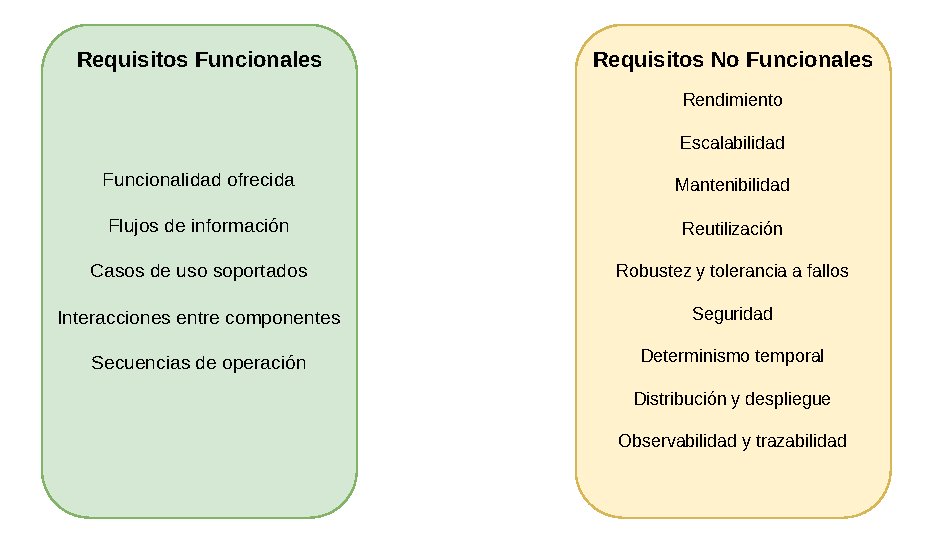
\includegraphics[width=\linewidth,height=0.45\textheight,keepaspectratio]{images/tema_1/requisitos.pdf}
\end{center}
\end{frame}

\begin{frame}{Qué es arquitectura software}
\small
\begin{columns}[T,onlytextwidth]
  \begin{column}{0.60\textwidth}
    \begin{itemize}
      \item Define elementos arquitectónicos: módulos, interfaces, mecanismos de comunicación y patrones (desacoplamiento, modularidad, jerarquía).
      \item Condiciona la evolución: integración de nuevos componentes, reutilización, testabilidad y contención de fallos.
      \item No existe una arquitectura universal: se diseña por compromisos y se valida contra el contexto y los requisitos.
    \end{itemize}
  \end{column}
  \begin{column}{0.40\textwidth}
    \centering
    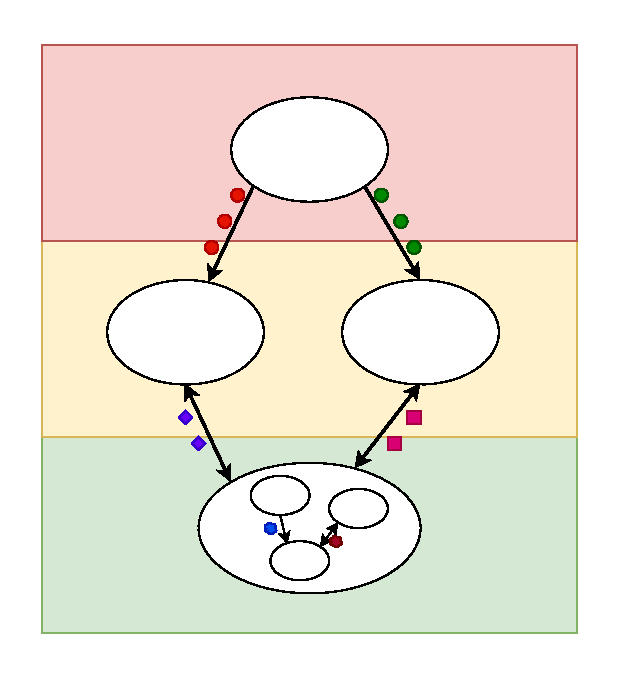
\includegraphics[width=\linewidth,height=0.70\textheight,keepaspectratio]{images/tema_1/arquitectura_abs.pdf}
  \end{column}
\end{columns}
\end{frame}

%-------------------------------------------------
\begin{frame}{Qué es arquitectura software en robótica}
\small
\begin{minipage}[t]{\linewidth}
\begin{itemize}
  \item Organización del software que permite al robot percibir, decidir y actuar en el mundo físico.
  \item Particularidades: entorno dinámico e incierto, datos sensoriales con caducidad, y actuación con consecuencias físicas.
  \item La arquitectura debe garantizar un comportamiento \textbf{coherente, robusto y seguro} ante incertidumbre, degradaciones y fallos.
  \item Adapta principios clásicos (modularidad, desacoplamiento, reutilización) a un dominio con requisitos \textbf{físicos y temporales}.
  \item Exige tratar explícitamente tiempo y concurrencia: latencia, sincronización, priorización y tolerancia a fallos.
\end{itemize}
\end{minipage}

\vfill
\begin{center}
  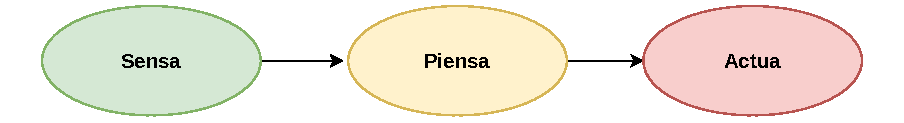
\includegraphics[width=0.5\linewidth,height=0.30\textheight,keepaspectratio]{images/tema_1/sense_think_act.pdf}
\end{center}
\end{frame}

\begin{frame}{Qué es arquitectura software en robótica}
\small
\begin{minipage}[t]{\linewidth}
\begin{itemize}
  \item Estructura funcional típica: percepción, modelado, planificación, control y supervisión, con dependencias fuertes.
  \item Define cómo fluye la información: \textbf{representaciones compartidas}, coordinación de comportamientos y decisiones \textbf{reactivas} vs. \textbf{deliberativas}.
  \item Debe ser \textbf{adaptable y extensible}: integrar nuevos sensores, sustituir algoritmos e incorporar capacidades sin reescribir el sistema.
  \item Requiere monitorización y trazabilidad: exponer estado interno y reconstruir decisiones para depurar, validar y asegurar.
\end{itemize}
\end{minipage}

\vfill
\begin{center}
  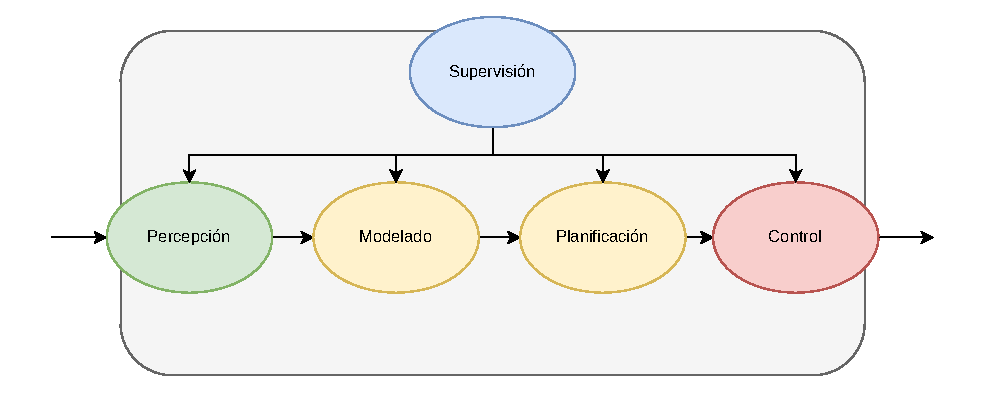
\includegraphics[width=\linewidth,height=0.33\textheight,keepaspectratio]{images/tema_1/sense_think_act_ext.pdf}
\end{center}
\end{frame}

%-------------------------------------------------
\begin{frame}{Middlewares de programación de robot: idea principal}
\small
\begin{itemize}
  \item Un middleware evita rehacer infraestructura: comunicación, abstracción de hardware y modelos de ejecución.
  \item Materializa la arquitectura: convierte interacciones y componentes definidos en diseño en comportamiento en ejecución.
  \item Condiciona decisiones arquitectónicas: acoplamiento posible, modelo de concurrencia, distribución y garantías temporales.
  \item Suele incluir: transporte de mensajes, descubrimiento, serialización, \emph{runtime}, herramientas de despliegue e introspección.
\end{itemize}

\vfill
\begin{center}
  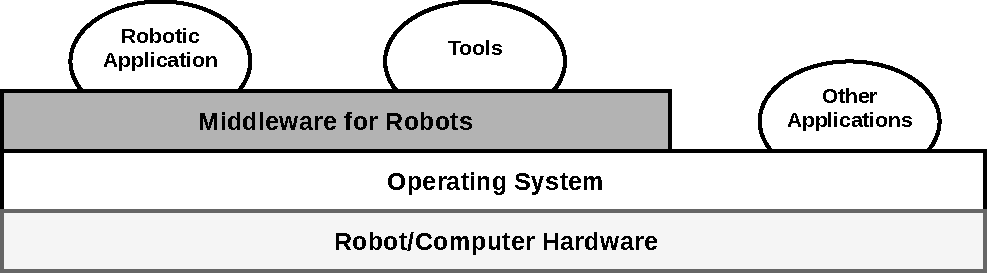
\includegraphics[width=0.6\linewidth,height=0.35\textheight,keepaspectratio]{images/tema_1/middleware_layers.pdf}
\end{center}
\end{frame}

%-------------------------------------------------
% \begin{frame}{Middlewares: ejemplos y rasgos arquitectónicos}
% \framesubtitle{Open-R (Aibo)}
% \small
% \begin{minipage}[t]{\linewidth}
% \begin{itemize}
%   \item \textbf{Open-R (Aibo):} tiempo real fuerte; arquitectura de objetos concurrentes (un \emph{thread} por objeto) y comunicación por mensajes tipados.
% \end{itemize}
% \end{minipage}

% \vfill
% \begin{center}
%   \includegraphics[width=0.5\linewidth,height=0.58\textheight,keepaspectratio]{images/tema_1/aiboware.png}
% \end{center}
% \end{frame}

% \begin{frame}{Middlewares: ejemplos y rasgos arquitectónicos}
% \framesubtitle{NaoQi (Nao/Pepper)}
% \small
% \begin{minipage}[t]{\linewidth}
% \begin{itemize}
%   \item \textbf{NaoQi (Nao/Pepper):} módulos preexistentes accesibles por \emph{proxies}; \emph{blackboard} interna y modelo multihilo gestionado por el middleware.
% \end{itemize}
% \end{minipage}

% \vfill
% \begin{center}
%   \includegraphics[width=\linewidth,height=0.58\textheight,keepaspectratio]{images/tema_1/naoqi.png}
% \end{center}
% \end{frame}

% \begin{frame}{Middlewares: ejemplos y rasgos arquitectónicos}
% \framesubtitle{Player/Stage}
% \small
% \begin{minipage}[t]{\linewidth}
% \begin{itemize}
%   \item \textbf{Player/Stage:} enfoque cliente--servidor; separación clara hardware--algoritmos y simulación 2D para reutilizar el mismo software.
% \end{itemize}
% \end{minipage}

% \vfill
% \begin{center}
%   \includegraphics[width=\linewidth,height=0.58\textheight,keepaspectratio]{images/tema_1/stage_playerv.jpg}
% \end{center}
% \end{frame}

% \begin{frame}{Middlewares: ejemplos y rasgos arquitectónicos}
% \framesubtitle{YARP}
% \small
% \begin{minipage}[t]{\linewidth}
% \begin{itemize}
%   \item \textbf{YARP:} comunicación por \emph{ports} tipados y conexiones dinámicas; favorece sistemas distribuidos y débilmente acoplados.
% \end{itemize}
% \end{minipage}

% \vfill
% \begin{center}
%   \includegraphics[width=\linewidth,height=0.28\textheight,keepaspectratio]{images/tema_1/yarp-logo-name.png}
% \end{center}
% \end{frame}

% \begin{frame}{Middlewares: ejemplos y rasgos arquitectónicos}
% \framesubtitle{Orocos}
% \small
% \begin{minipage}[t]{\linewidth}
% \begin{itemize}
%   \item \textbf{Orocos:} orientación a control en tiempo real; componentes con \emph{ports} y ejecución determinista para capas de bajo nivel.
% \end{itemize}
% \end{minipage}

% \vfill
% \begin{center}
%   \includegraphics[width=\linewidth,height=0.38\textheight,keepaspectratio]{images/tema_1/orocos.png}
% \end{center}
% \end{frame}

%-------------------------------------------------
\begin{frame}{ROS y ROS 2 como \emph{middleware} de facto}
\small
\begin{itemize}
  \item ROS/ROS~2 es el estándar de facto: comunidad muy amplia y ecosistema de paquetes reutilizables (navegación, manipulación, percepción, simulación)
  \item ROS~2 amplía ROS para sistemas reales: distribución nativa, multi-robot y soporte de tiempo real sobre DDS
  \item Impacto arquitectónico: reutilización de paquetes y convenciones de la comunidad condicionan estructura y decisiones de integración
  \item Aplicaciones: desde prototipos de investigación hasta robots industriales, móviles, de servicio y vehículos autónomos
\end{itemize}

\vfill
\begin{center}
  
\includegraphics[width=0.55\linewidth,height=0.38\textheight,keepaspectratio]{images/tema_1/ros2.png}
\end{center}
\end{frame}

%=================================================
\section{ROS 2}
%=================================================

%-------------------------------------------------
\begin{frame}{ROS 2 como materialización de una arquitectura software robótica}
\small
\begin{itemize}
  \item ROS~2 no impone una arquitectura funcional: proporciona primitivas para implementar la arquitectura que el ingeniero diseña
  \item Modelo arquitectónico: nodos desacoplados que interactúan mediante topics, servicios y acciones
  \item Integra requisitos robóticos como elementos centrales: tiempo, concurrencia y distribución desde el diseño del \emph{runtime}
  \item Incorpora observabilidad y trazabilidad: introspección del sistema y registro de eventos para cerrar el ciclo diseño--ejecución
\end{itemize}

\vfill
\begin{center}
  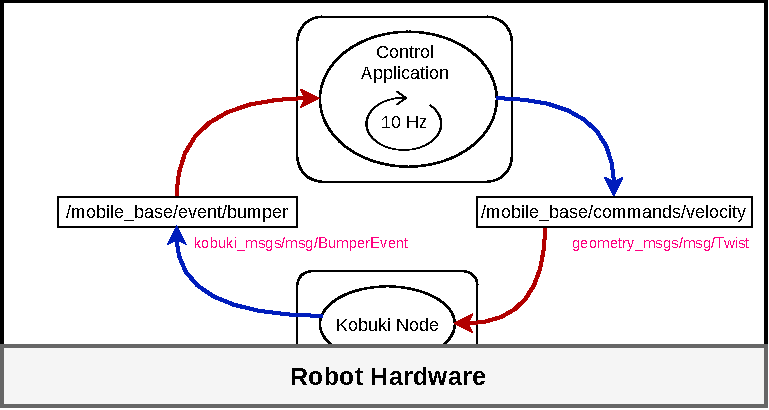
\includegraphics[width=\linewidth,height=0.3\textheight,keepaspectratio]{images/tema_1/comp_graph_0.pdf}
\end{center}
\end{frame}

%-------------------------------------------------
\begin{frame}{Componentes, procesos y comunicación en ROS 2}
\small
\begin{itemize}
  \item \textbf{Nodo} como unidad arquitectónica: encapsula responsabilidades y delimita interfaces
  \item \textbf{Proceso} como decisión de despliegue: aislamiento y robustez frente a latencia y consumo de recursos
  \item \textbf{Topics} para datos asíncronos (desacoplamiento productor--consumidor) y flujos continuos
  \item \textbf{Servicios} para peticiones puntuales síncronas; \textbf{acciones} para tareas largas con \emph{feedback}
  \item Elegir mecanismo de comunicación es una decisión arquitectónica: define dependencias, acoplamiento y ritmo del sistema
\end{itemize}
\end{frame}

\begin{frame}{Componentes, procesos y comunicación en ROS 2}

\small
\vfill
\begin{columns}[T,onlytextwidth]
  \begin{column}{0.50\textwidth}
    \centering
    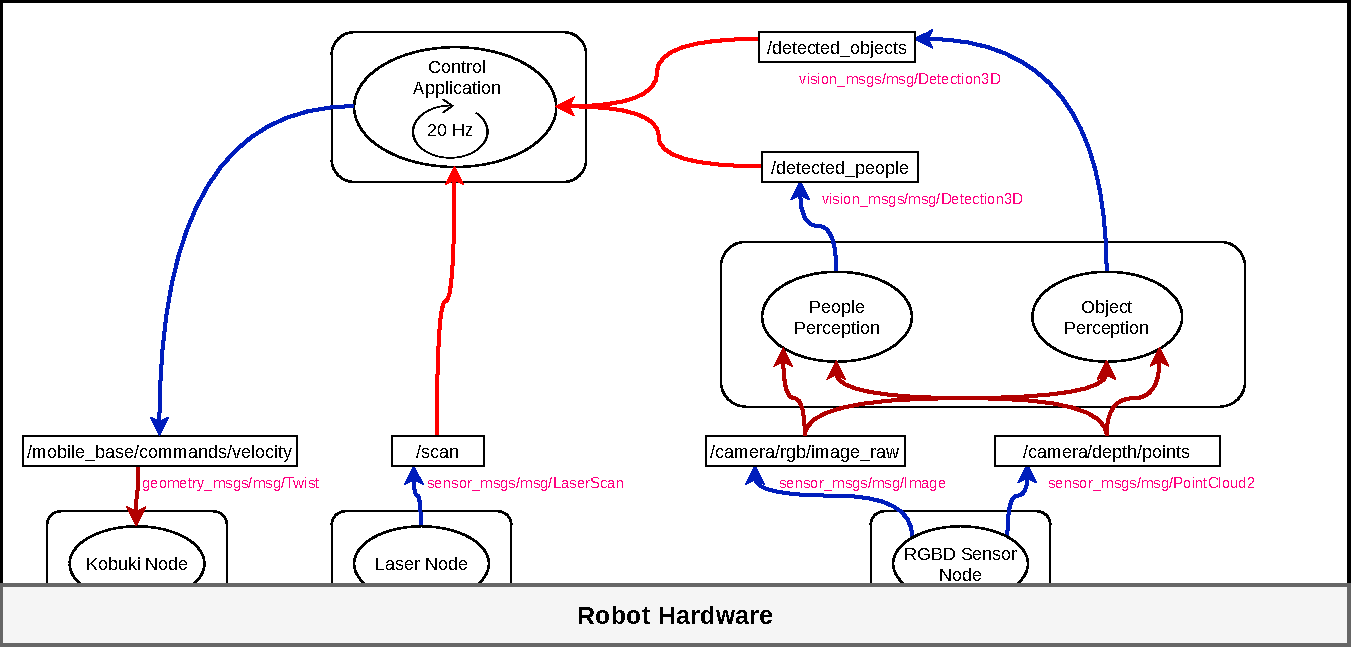
\includegraphics[width=\linewidth,height=0.6\textheight,keepaspectratio]{images/tema_1/comp_graph_2.pdf}
  \end{column}
  \begin{column}{0.50\textwidth}
    \centering
    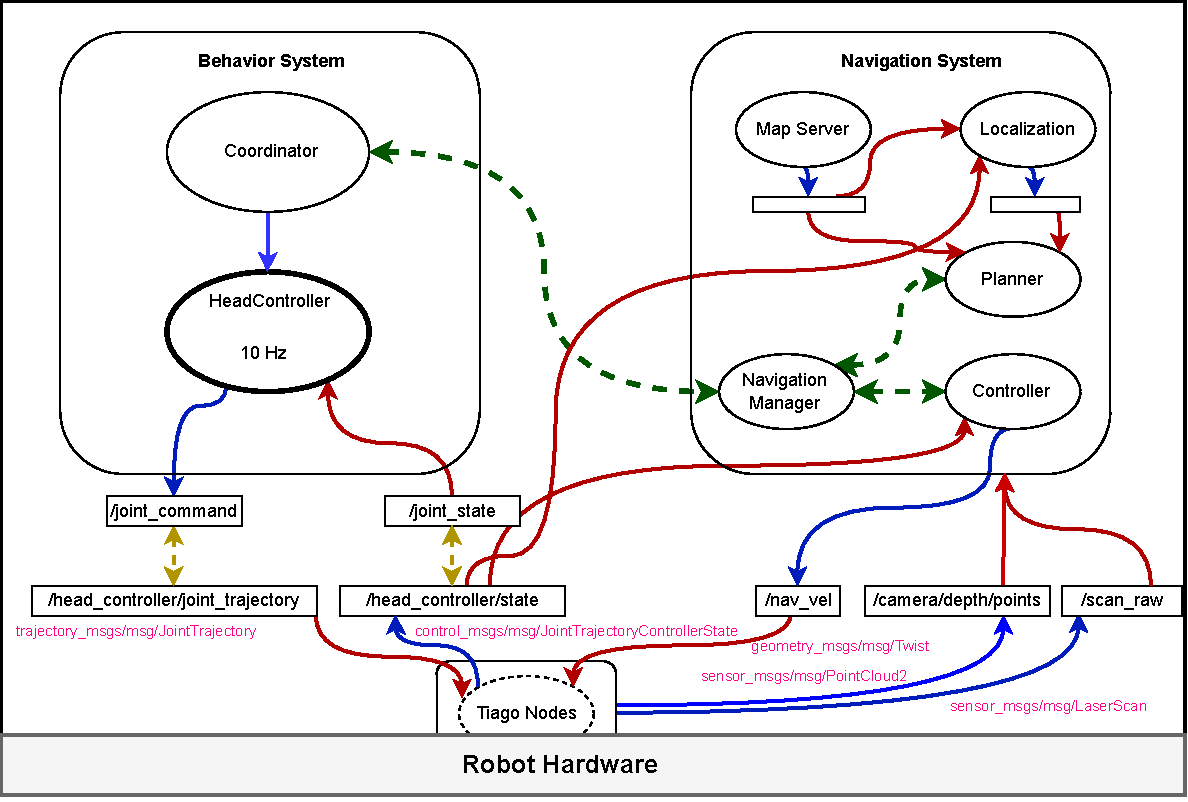
\includegraphics[width=\linewidth,height=0.6\textheight,keepaspectratio]{images/tema_1/comp_graph_3.pdf}
  \end{column}
\end{columns}
\vfill
\end{frame}

%-------------------------------------------------
\begin{frame}{Componentes, procesos y comunicación en ROS 2}
\small
\begin{itemize}
  \item Modelo orientado a eventos: los componentes reaccionan a datos, temporizadores y peticiones externas
  \item Concurrencia de actividades: percepción, procesamiento, control y supervisión progresan de forma solapada
  \item Diseño distribuido por naturaleza: nodos en procesos y máquinas distintas con comunicación transparente en red
  \item \textbf{Introspección} del grafo y \textbf{monitorización}: nodos, interfaces, conexiones y salud del sistema en ejecución
  \item \textbf{Logging} y \textbf{trazas} del \emph{runtime} para reconstruir decisiones, validar comportamiento y facilitar depuración
\end{itemize}
\end{frame}

%=================================================
\section{Uso práctico de ROS 2}
%=================================================

%-------------------------------------------------
\begin{frame}{Workspace, paquetes, underlay y overlay}
\small
\begin{itemize}
  \item ROS~2 organiza el software en \emph{workspaces} con código, compilación y ejecución
  \item El paquete es la unidad básica de distribución en ROS~2
  \item El \textbf{underlay} contiene los paquetes ROS~2 instalados en el sistema (/opt/ros/<distro>)
  \item El \textbf{overlay} es el workspace del usuario con paquetes propios o de terceros
\end{itemize}
\vfill
\begin{center}
  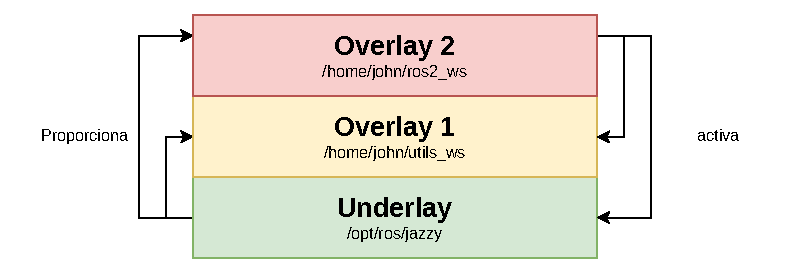
\includegraphics[width=0.9\linewidth]{images/tema_1/overlays.pdf}
\end{center}
\end{frame}

%-------------------------------------------------
\begin{frame}[fragile]{Activación del entorno y persistencia}
\small
\begin{itemize}
  \item Activar ROS~2 significa configurar variables de entorno del sistema
  \item La activación se realiza mediante el script \texttt{setup.bash} que se genera en el directorio \texttt{install} del workspace
  \item Primero se activa el underlay de ROS~2 instalado
  \item Después se activa el overlay del workspace del usuario
  \item Sin activación, ROS~2 no puede localizar paquetes ni ejecutables
  \item La activación puede hacerse persistente mediante el fichero \texttt{.bashrc}
\end{itemize}
\vspace{2mm}
\begin{terminal}
source /opt/ros/jazzy/setup.bash
source install/setup.bash
\end{terminal}
\end{frame}

%-------------------------------------------------
\begin{frame}[fragile]{Compilación del workspace}
\small
\begin{itemize}
  \item Un workspace es un directorio que contiene múltiples paquetes ROS~2 bajo su carpeta \texttt{src}
  \item Los workspaces se compilan con la herramienta colcon
  \item La compilación siempre se realiza desde el directorio raíz del workspace
  \item La opción \texttt{--symlink-install} evita copias innecesarias de ficheros (recomendada)
  \item Crea el directorio \texttt{install} con los paquetes compilados y configurados
  \item Tras compilar, es necesario recargar el entorno para activar los nuevos paquetes
  \item Se limpia borrando \texttt{build}, \texttt{install} y \texttt{log} si es necesario
\end{itemize}
\vspace{2mm}
\begin{terminal}
colcon build --symlink-install
\end{terminal}
\end{frame}

%-------------------------------------------------
\begin{frame}[fragile]{Herramientas de línea de comandos (ros2cli)}
\small
\begin{itemize}
  \item \texttt{ros2cli} permite inspeccionar y controlar sistemas en ejecución
  \item El comando base sigue el patrón mostrado a continuación
  \item Cada comando se asocia a un dominio del sistema
  \item Permite analizar sistemas sin modificar el código
  \item El autocompletado con TAB facilita la exploración interactiva
\end{itemize}
\vspace{2mm}
\begin{terminal}
ros2 <comando> <verbo>

ros2 node list
ros2 topic list
ros2 topic echo /scan
\end{terminal}
\end{frame}

%-------------------------------------------------
\begin{frame}[fragile]{Ejecución de nodos en ROS~2}
\small
\begin{itemize}
  \item Un nodo es la unidad básica de ejecución en ROS~2
  \item El subcomando \textbf{run} ejecuta un único nodo directamente
  \item No es necesario conocer la ruta del ejecutable
  \item El subcomando \textbf{launch} ejecuta múltiples nodos coordinados
  \item Los launch files gestionan parámetros, remapeos y dependencias
\end{itemize}
\vspace{2mm}
\begin{terminal}
ros2 run <paquete> <ejecutable>
ros2 launch <paquete> <archivo.launch.py>
\end{terminal}
\end{frame}

%-------------------------------------------------
\begin{frame}{Interfaces y parámetros}
\small
\begin{itemize}
  \item Las interfaces definen cómo se comunican los nodos
  \item Incluyen mensajes, servicios y acciones
  \item Los parámetros permiten configurar nodos sin modificar código
  \item Cambiar parámetros altera el comportamiento en tiempo de ejecución
  \item Comprender interfaces y parámetros es clave para analizar sistemas ROS~2
\end{itemize}
\end{frame}

%-------------------------------------------------
\begin{frame}[fragile]{Paquetes y ejecutables}
\small
\begin{itemize}
  \item Un paquete puede contener nodos, librerías, interfaces y configuraciones
  \item Mostrar paquetes disponibles y descubrir ejecutables
  \item Es clave para explorar sistemas sin documentación previa
\end{itemize}
\vspace{2mm}
\begin{terminal}
ros2 pkg list
ros2 pkg executables <paquete> # ejemplo: ros2 pkg executables demo_nodes_cpp
\end{terminal}
\end{frame}

%-------------------------------------------------
\begin{frame}[fragile]{Nodos y grafo de computación}
\small
\begin{itemize}
  \item Los nodos (hay que lanzarlos) se comunican mediante topics, servicios y acciones
  \item Listar nodos activos e inspeccionar sus interfaces y parámetros
  \item Permite entender el papel de cada nodo en el sistema
  \item Es fundamental para analizar el grafo de computación del robot
\end{itemize}
\vspace{2mm}
\begin{terminal}
ros2 run <paquete> <ejecutable> # ejemplo: ros2 run demo_nodes_cpp talker
ros2 node list
ros2 node info <nodo>
\end{terminal}
\end{frame}

%-------------------------------------------------
\begin{frame}[fragile]{Topics e inspección de datos}
\small
\begin{itemize}
  \item Los topics son canales asíncronos de intercambio de datos
  \item Listar topics, consultar tipos y ver datos en tiempo real
  \item Es la forma más rápida de verificar que un nodo funciona
\end{itemize}
\vspace{2mm}
\begin{terminal}
ros2 topic list
ros2 topic type /chatter
ros2 topic echo /chatter
\end{terminal}
\end{frame}

%-------------------------------------------------
\begin{frame}[fragile]{Interfaces y parámetros en práctica}
\small
\begin{itemize}
  \item Inspeccionar interfaces y parámetros desde terminal.
  \item Los parámetros son esenciales en simulación y depuración.
\end{itemize}
\vspace{2mm}
\begin{terminal}
ros2 interface list
ros2 interface show <interfaz> # ejemplo: ros2 interface show std_msgs/msg/String

ros2 param list
ros2 param get <nodo> <parametro>
ros2 param set <nodo> <parametro> <valor>
\end{terminal}
\end{frame}

%-------------------------------------------------
\begin{frame}[fragile]{Flujo típico de trabajo en la práctica}
\small
\begin{itemize}
  \item Activar underlay y overlay
  \item Compilar el workspace
  \item Recargar el entorno tras la compilación
  \item Ejecutar nodos o simuladores
  \item Analizar el sistema con \texttt{ros2cli} y RViz2
\end{itemize}
\vspace{2mm}
\begin{terminal}
source /opt/ros/jazzy/setup.bash
source install/setup.bash

colcon build --symlink-install
source install/setup.bash
ros2 launch <paquete> <archivo.launch.py>
\end{terminal}
\end{frame}

%-------------------------------------------------
\begin{frame}[fragile]{Simulador del Kobuki}
\small
\begin{itemize}
  \item El simulador se distribuye como paquetes ROS~2 que se compilan en el overlay
  \item El código fuente se obtiene clonando el repositorio en \texttt{src}
  \item Tras compilar, hay que recargar el overlay para que ROS~2 encuentre el paquete
  \item Se lanza con un \texttt{launch} (con o sin interfaz gráfica)
\end{itemize}
\vspace{2mm}
\begin{terminal}
git clone https://github.com/IntelligentRoboticsLabs/ASR-Software.git
colcon build --symlink-install
source install/setup.bash

ros2 launch kobuki simulation.launch.py
# Alternativa sin GUI (equipos con pocos recursos)
ros2 launch kobuki simulation.launch.py gui:=false
\end{terminal}
\end{frame}

%-------------------------------------------------
\begin{frame}{Visualización con RViz2}
\small
\begin{itemize}
  \item RViz2 es la herramienta estándar de visualización en ROS~2
  \item Permite inspeccionar sensores, mapas y estados del robot
  \item Es necesario fijar correctamente el \texttt{Fixed Frame}
  % \item Los datos del láser se visualizan mediante \texttt{LaserScan}
  \item Confirma visualmente que el sistema funciona correctamente
\end{itemize}
\end{frame}




\end{document}
